\section{Архитектура}

\subsection{Ствол}

Предобученный химический энкодер $f_\varphi:\ \text{SMILES} \to z \in \mathbb{R}^d$. Организаторы выложили
свои веса (CheMeleon, предобученный D-MPNN, и chemprop-foundation), плюс доступны Minimol и графовые
трансформеры. Ансамблируем по семействам претрейна, а не по сидам одного семейства: ошибки разных
семейств коррелируют слабее, и ансамбль из четырёх разных архитектур даёт больше, чем из восьми запусков
одной. Дообучение через LoRA-адаптеры, чтобы 6.5 тысяч меток кривых не переписали претрейн, обученный
на миллионах молекул.

\subsection{Связь между ферментами: коррегионализация}
\label{sec:icm}

Ферментов четыре, и надо решить, как их связать. Очевидные способы не годятся. Четыре независимые модели:
2C9 не пользуется 2335 метками 3A4, хотя они меряют почти одно и то же. Одна общая голова: 2D6 тянет
в сторону остальных трёх, а он с ними не коррелирует. Общий ствол и четыре независимые головы уже лучше,
но связь между задачами остаётся неявной.

Коррегионализация --- термин из геостатистики: совместное моделирование нескольких величин, измеренных
в одних точках, через общую структуру плюс отдельную матрицу связей между величинами. Простейший вариант,
intrinsic coregionalization model, выносит эту матрицу в явный параметр.

Голова линейная поверх общего представления:
\begin{equation}
\pi_{m,e} = w_e^{\top} g(z_m) + b_e,
\qquad W = [\,w_1\ w_2\ w_3\ w_4\,] \in \mathbb{R}^{d\times 4} .
\label{eq:head}
\end{equation}

Вся связь между ферментами сидит в углах между столбцами $W$: если $w_2$ и $w_4$ смотрят почти в одну
сторону, модели 2C9 и 3A4 читают представление одинаково. Матрица этих углов
\begin{equation}
B = W^{\top}W \in \mathbb{R}^{4\times 4}, \qquad B_{ee'} = w_e^{\top} w_{e'} ,
\end{equation}
и на неё навязывается структура «несколько общих осей плюс своё у каждого»:
\begin{equation}
B \;\approx\; LL^{\top} + \operatorname{diag}(\kappa),
\qquad L \in \mathbb{R}^{4\times r},\quad r = 2 .
\label{eq:icm}
\end{equation}

Строка $e$ матрицы $L$ говорит, насколько фермент участвует в каждой из $r$ общих осей; $LL^{\top}$ ---
общая часть ковариации ранга $r$; $\kappa_e$ --- специфичная часть фермента, то, что есть только у него.
Это обычная факторная модель: $r$ общих механизмов узнавания плюс идиосинкразия.

\begin{figure}[htbp]\centering
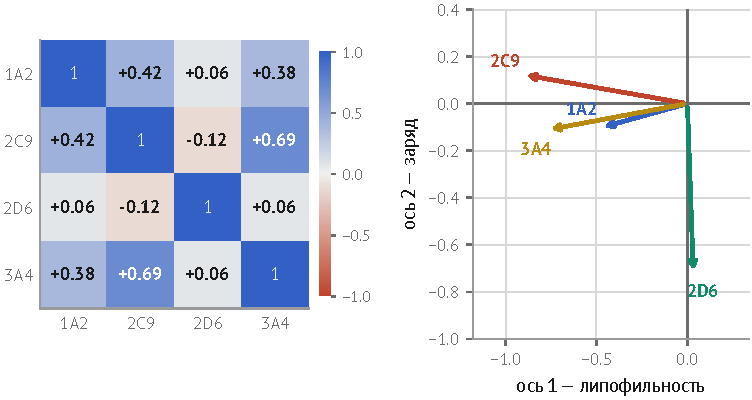
\includegraphics{fig/corr}
\caption{Слева --- ранговая корреляция $\pic$ между ферментами, посчитанная по общим соединениям
(от 230 пар у 2C9--2D6 до 473 у 2C9--3A4). Справа --- нагрузки факторной модели ранга 2 на те же данные:
каждая стрелка показывает, насколько фермент участвует в каждой из двух общих осей. Первая ось нагружает
2C9, 3A4 и слабее 1A2, на 2D6 стоит на нуле; вторая ось --- почти исключительно 2D6.}
\label{fig:corr}
\end{figure}

Данные говорят то же, что раздел~\ref{sec:isoforms}: 2C9 и 3A4 идут в паре ($\rho = 0.688$),
а 2D6 ортогонален всем троим ($0.059$, $-0.120$, $0.056$). Матрица положительно определена, минимальное собственное число 0.287, так что
раскладывать её можно. Нагрузки: ось 1 --- 2C9 $-0.907$, 3A4 $-0.773$, 1A2 $-0.480$, 2D6 $+0.033$;
ось 2 --- 2D6 $-0.726$, остальные около нуля. Специфичные части $\kappa$: 0.759, 0.161, 0.472, 0.390.

Первая ось --- липофильная промискуитетность: крупные жирные молекулы садятся в широкие карманы 2C9 и 3A4.
Вторая --- 2D6 с его солевым мостиком. Общая голова тянула бы 2D6 по первой оси и портила бы его.

Про ранг надо помнить вот что. При четырёх задачах внедиагональ содержит шесть чисел,
а нагрузки ранга 2 дают $4\times 2 = 8$ параметров минус одна степень свободы на вращение, то есть семь.
Модель насыщена: ранг 2 воспроизводит внедиагональ точно не потому, что угадал структуру, а потому что
параметров хватает. По-настоящему ограничивает только ранг 1, и он промахивается максимум на 0.10, причём
весь промах приходится на 2D6. Так что структура ранга 2 --- не сжатие, а способ задать приор и инициализацию. Польза проявится, когда
$B$ будет тянуть головы во время обучения, а не в самой аппроксимации матрицы четыре на четыре.

\paragraph{Регуляризационный член.} Задача --- не дать столбцам $W$ разъехаться в произвольные углы,
когда у фермента мало меток, и притянуть матрицу связей к тому, что видно в данных:
\begin{equation}
\Omega(W) \;=\;
\frac{\lambda_1}{2}\,\bigl\| \rho(W^{\top}W) - \widehat{\rho} \bigr\|_F^2
\;+\;
\frac{\lambda_2}{2}\,\|W\|_F^2 ,
\qquad
\rho(B) = D^{-1/2} B D^{-1/2},\ \ D = \operatorname{diag}(B) .
\label{eq:omega}
\end{equation}

Первое слагаемое: строим $B$, нормируем в корреляционную матрицу, вычитаем эмпирическую $\widehat{\rho}$,
складываем квадраты разностей. Нормировка нужна потому, что притягивать надо \emph{углы}, а не длины
столбцов --- длина отвечает за масштаб предсказания и настраивается данными. Второе --- обычная усадка весов.
Норма Фробениуса $\|A\|_F = \sqrt{\sum_{ij}A_{ij}^2}$ --- евклидова длина матрицы, вытянутой в строку.

Почему именно так, а не поэлементный штраф на $W$. Матрица $W$ определена не однозначно: умножение справа
на любую ортогональную $Q$ не меняет ни $W^{\top}W$, ни предсказания. Регуляризатор обязан обладать той же
симметрией, иначе он штрафует за выбор системы координат, а не за содержание. Обе величины в
\eqref{eq:omega} проходят через $W$ только в виде $W^{\top}W$, поэтому симметрию сохраняют; поэлементный
штраф --- нет.

Низкий ранг входит не штрафом, а параметризацией. Практически проще держать не $W$ со сложным штрафом,
а сразу $L$ и $\kappa$ и строить головы из них:
\begin{equation}
\pi_{m,e} = L_{e\cdot}\, U^{\top} g(z_m) \;+\; \sqrt{\kappa_e}\; s_e^{\top} g(z_m) \;+\; b_e ,
\label{eq:headfac}
\end{equation}
где $U \in \mathbb{R}^{d\times 2}$ --- проекция на общие оси, общая для всех ферментов, а $s_e$ --- вектор
специфичного направления фермента. Тогда $B = LL^{\top} + \operatorname{diag}(\kappa)$ выполняется
по построению, штраф за ранг не нужен, а от \eqref{eq:omega} остаётся притяжение к $\widehat{\rho}$
плюс усадка. Инициализация $L$ и $\kappa$ --- из факторного разложения эмпирической матрицы, причём
именно факторным анализом с итеративной оценкой общностей: наивное собственное разложение полной матрицы
с единицами на диагонали искажает внедиагональные элементы до 0.23, потому что факторы начинают гнаться
за диагональю.

Проверять надо две вещи. Положить $\lambda_1 = 0$ и посмотреть, куда уедет выученная матрица связей
от эмпирической: если далеко, значит либо в представлении есть структура, которой нет в сырых корреляциях,
либо голова переобучается. И сравнить с четырьмя независимыми головами на тех же разбиениях.

\subsection{Механистический блок}

30 признаков, описанных в разделе~\ref{sec:d6}, конкатенируются с $z_m$ либо подаются через FiLM ---
то есть модулируют активации ствола, а не просто дописываются в конец вектора.

Зачем блок нужен, если по метрике он почти ничего не даёт. По ранжированию он избирателен так, как
предсказывает химия, и это подтверждено бутстрапом; модель на одних этих 30 числах воспроизводит большую
часть ранжирующей способности на 2D6 и меньше половины на остальных. Вдобавок он заметно стабилизирует
модель (раздел~\ref{sec:proto}). Считается блок за секунду.

\subsection{Канал артефактов пробы}
\label{sec:artifact}

Как описано в разделе~\ref{sec:bio}, 1A2, 2C9 и 3A4 читаются по флуоресценции, а 2D6 ---
масс-спектрометрией, и собственная флуоресценция соединения или тушение сигнала дают ложное
«ингибирование» только в первых трёх. Это конфаундер, общий для трёх эндпойнтов и отсутствующий
у четвёртого, и он частично объясняет, почему 1A2, 2C9 и 3A4 коррелируют между собой.

Добавляем скалярный признак-помеху (протяжённость сопряжения, известные хромофорные каркасы) с обучаемым
коэффициентом, входящий только в три флуоресцентных эндпойнта. Это поправка на конфаундер с известной структурой, а не ещё один признак в общую кучу: модель получает
возможность объяснить часть общей вариации артефактом, а не химией.

\subsection{Головы}

\begin{itemize}
\item $\pi$-голова --- линейная поверх \eqref{eq:headfac}, выход в $\mathbb{R}$.
\item $(\sigma^-, \sigma^+)$-головы --- гетероскедастичные, через softplus; обучаются через
\eqref{eq:split}. Границы интервалов лежат в данных и обычно никем не используются, а решающему слою
они нужны.
\item $E$ --- константа на фермент, по итогам раздела~\ref{sec:ident}, плюс опциональная штрафуемая поправка.
\item $\Delta$-голова --- softplus, отдельная. Не разность двух независимых регрессий: шум двух плеч
коррелирован и частично сокращается в разности, поэтому предсказывать сдвиг напрямую точнее. Измерено:
0.255 против 0.323 по MCC на 3A4 в пользу отдельной головы.
\end{itemize}
